\documentclass[twoside]{book}

% Packages required by doxygen
\usepackage{fixltx2e}
\usepackage{calc}
\usepackage{doxygen}
\usepackage[export]{adjustbox} % also loads graphicx
\usepackage{graphicx}
\usepackage[utf8]{inputenc}
\usepackage{makeidx}
\usepackage{multicol}
\usepackage{multirow}
\PassOptionsToPackage{warn}{textcomp}
\usepackage{textcomp}
\usepackage[nointegrals]{wasysym}
\usepackage[table]{xcolor}

% Font selection
\usepackage[T1]{fontenc}
\usepackage[scaled=.90]{helvet}
\usepackage{courier}
\usepackage{amssymb}
\usepackage{sectsty}
\renewcommand{\familydefault}{\sfdefault}
\allsectionsfont{%
  \fontseries{bc}\selectfont%
  \color{darkgray}%
}
\renewcommand{\DoxyLabelFont}{%
  \fontseries{bc}\selectfont%
  \color{darkgray}%
}
\newcommand{\+}{\discretionary{\mbox{\scriptsize$\hookleftarrow$}}{}{}}

% Page & text layout
\usepackage{geometry}
\geometry{%
  a4paper,%
  top=2.5cm,%
  bottom=2.5cm,%
  left=2.5cm,%
  right=2.5cm%
}
\tolerance=750
\hfuzz=15pt
\hbadness=750
\setlength{\emergencystretch}{15pt}
\setlength{\parindent}{0cm}
\setlength{\parskip}{3ex plus 2ex minus 2ex}
\makeatletter
\renewcommand{\paragraph}{%
  \@startsection{paragraph}{4}{0ex}{-1.0ex}{1.0ex}{%
    \normalfont\normalsize\bfseries\SS@parafont%
  }%
}
\renewcommand{\subparagraph}{%
  \@startsection{subparagraph}{5}{0ex}{-1.0ex}{1.0ex}{%
    \normalfont\normalsize\bfseries\SS@subparafont%
  }%
}
\makeatother

% Headers & footers
\usepackage{fancyhdr}
\pagestyle{fancyplain}
\fancyhead[LE]{\fancyplain{}{\bfseries\thepage}}
\fancyhead[CE]{\fancyplain{}{}}
\fancyhead[RE]{\fancyplain{}{\bfseries\leftmark}}
\fancyhead[LO]{\fancyplain{}{\bfseries\rightmark}}
\fancyhead[CO]{\fancyplain{}{}}
\fancyhead[RO]{\fancyplain{}{\bfseries\thepage}}
\fancyfoot[LE]{\fancyplain{}{}}
\fancyfoot[CE]{\fancyplain{}{}}
\fancyfoot[RE]{\fancyplain{}{\bfseries\scriptsize Generated by Doxygen }}
\fancyfoot[LO]{\fancyplain{}{\bfseries\scriptsize Generated by Doxygen }}
\fancyfoot[CO]{\fancyplain{}{}}
\fancyfoot[RO]{\fancyplain{}{}}
\renewcommand{\footrulewidth}{0.4pt}
\renewcommand{\chaptermark}[1]{%
  \markboth{#1}{}%
}
\renewcommand{\sectionmark}[1]{%
  \markright{\thesection\ #1}%
}

% Indices & bibliography
\usepackage{natbib}
\usepackage[titles]{tocloft}
\setcounter{tocdepth}{3}
\setcounter{secnumdepth}{5}
\makeindex

% Hyperlinks (required, but should be loaded last)
\usepackage{ifpdf}
\ifpdf
  \usepackage[pdftex,pagebackref=true]{hyperref}
\else
  \usepackage[ps2pdf,pagebackref=true]{hyperref}
\fi
\hypersetup{%
  colorlinks=true,%
  linkcolor=blue,%
  citecolor=blue,%
  unicode%
}

% Custom commands
\newcommand{\clearemptydoublepage}{%
  \newpage{\pagestyle{empty}\cleardoublepage}%
}

\usepackage{caption}
\captionsetup{labelsep=space,justification=centering,font={bf},singlelinecheck=off,skip=4pt,position=top}

%===== C O N T E N T S =====

\begin{document}

% Titlepage & ToC
\hypersetup{pageanchor=false,
             bookmarksnumbered=true,
             pdfencoding=unicode
            }
\pagenumbering{alph}
\begin{titlepage}
\vspace*{7cm}
\begin{center}%
{\Large Fuse\+To\+Euler }\\
\vspace*{1cm}
{\large Generated by Doxygen 1.8.13}\\
\end{center}
\end{titlepage}
\clearemptydoublepage
\pagenumbering{roman}
\tableofcontents
\clearemptydoublepage
\pagenumbering{arabic}
\hypersetup{pageanchor=true}

%--- Begin generated contents ---
\chapter{Fuse\+To\+Euler Main}
\label{index}\hypertarget{index}{}\hypertarget{index_intro_sec}{}\section{Introduction}\label{index_intro_sec}
\begin{DoxyParagraph}{}
Many Real\+Sense cameras come with an embedded 6\+D\+OF Inertial Motion Unit (I\+MU) which measures rotation with a gyroscope and acceleration with an accelerometer. Unfortunately, with the exception of the Real\+Sense T265 tracking camera, this data is unfused, meaning that the data from each is N\+OT used to compensate for noise in the other. For example, when used naïvely, the raw orientation data is affected by any camera motion because there is no inherent way for the sensor to know whether an applied force is from gravity or another motive force. 
\end{DoxyParagraph}
\begin{DoxyParagraph}{}
Fusion algorithms \char`\"{}merge\char`\"{} the telemetry from independent sensor streams to create more stable results. 
\end{DoxyParagraph}
\begin{DoxyParagraph}{}
The Madgwick algorithm, named after Sebastian Madgwick who developed this algorithm in 2009, is one of the most popular ones. Fortunately for us, there is an open source library which implements this algorithm, ready to plunk into our code. In this tutorial, I will outline how to use it to derive the Euler orientation from the Real\+Sense gyroscope and accelerometer data. 
\end{DoxyParagraph}
\begin{DoxyParagraph}{}
I am programming in C/\+C++ on a Jetson A\+GX Xavier and using a Real\+Sense L515 Li\+D\+AR camera. 
\end{DoxyParagraph}
\begin{DoxyParagraph}{}
If you haven\textquotesingle{}t set up {\ttfamily librealsense2} yet, please see this \href{https://www.notion.so/How-to-install-librealsense-and-pylibrealsense-on-Jetson-5b909aeb1b6c409fb21464f2db869d41}{\tt tutorial} on installing it. 
\end{DoxyParagraph}
\hypertarget{index_download_sec}{}\section{Obtaining the Madgwick Library}\label{index_download_sec}
\begin{DoxyParagraph}{}
Clone the repo from github. 
\begin{DoxyCode}
cd ~/Documents
git clone https://github.com/xioTechnologies/Fusion.git Fusion-master
\end{DoxyCode}
 
\end{DoxyParagraph}
\begin{DoxyParagraph}{}
I did not create a library from this source, but rather compiled and linked the source code directly into my program. 
\end{DoxyParagraph}
\begin{DoxyParagraph}{}
Copy or move the Fusion directory from Fusion-\/master to your project directory. My project is contained in a folder named \char`\"{}\+Fuse\+To\+Euler\char`\"{}. 
\begin{DoxyCode}
mkdir FuseToEuler
cp -R Fusion-master/Fusion FuseToEuler
\end{DoxyCode}
 
\end{DoxyParagraph}

\chapter{Fuse\+To\+Euler}
\label{md_README}
\Hypertarget{md_README}
Demonstration of Madgwick Fusion on Real\+Sense I\+MU telemetry 
\chapter{Class Index}
\section{Class List}
Here are the classes, structs, unions and interfaces with brief descriptions\+:\begin{DoxyCompactList}
\item\contentsline{section}{\hyperlink{classException}{Exception} }{\pageref{classException}}{}
\item\contentsline{section}{\hyperlink{classIMUFusion}{I\+M\+U\+Fusion} \\*A class to encapsulate Madgwick Fusion access }{\pageref{classIMUFusion}}{}
\item\contentsline{section}{\hyperlink{classRealFusion}{Real\+Fusion} \\*A class to encapsulate librealsense2 and Fusion access }{\pageref{classRealFusion}}{}
\end{DoxyCompactList}

\chapter{File Index}
\section{File List}
Here is a list of all documented files with brief descriptions\+:\begin{DoxyCompactList}
\item\contentsline{section}{{\bfseries Exception.\+hpp} }{\pageref{Exception_8hpp}}{}
\item\contentsline{section}{\hyperlink{IMUFusion_8cpp}{I\+M\+U\+Fusion.\+cpp} \\*Fuse\+To\+Euler shows how to incorporate Sebastian Madgwick\textquotesingle{}s sensor fusion library to fuse raw I\+MU gyroscope and accelerometer telemetry from Real\+Sense cameras }{\pageref{IMUFusion_8cpp}}{}
\item\contentsline{section}{\hyperlink{IMUFusion_8hpp}{I\+M\+U\+Fusion.\+hpp} \\*Fuse\+To\+Euler shows how to incorporate Sebastian Madgwick\textquotesingle{}s sensor fusion library to fuse raw I\+MU gyroscope and accelerometer telemetry from Real\+Sense cameras }{\pageref{IMUFusion_8hpp}}{}
\item\contentsline{section}{\hyperlink{main_8cpp}{main.\+cpp} \\*Fuse\+To\+Euler shows how to incorporate Sebastian Madgwick\textquotesingle{}s sensor fusion library to fuse raw I\+MU gyroscope and accelerometer telemetry from Real\+Sense cameras }{\pageref{main_8cpp}}{}
\item\contentsline{section}{\hyperlink{RealFusion_8cpp}{Real\+Fusion.\+cpp} \\*Fuse\+To\+Euler shows how to incorporate Sebastian Madgwick\textquotesingle{}s sensor fusion library to fuse raw I\+MU gyroscope and accelerometer telemetry from Real\+Sense cameras }{\pageref{RealFusion_8cpp}}{}
\item\contentsline{section}{\hyperlink{RealFusion_8hpp}{Real\+Fusion.\+hpp} \\*Fuse\+To\+Euler shows how to incorporate Sebastian Madgwick\textquotesingle{}s sensor fusion library to fuse raw I\+MU gyroscope and accelerometer telemetry from Real\+Sense cameras }{\pageref{RealFusion_8hpp}}{}
\end{DoxyCompactList}

\chapter{Class Documentation}
\hypertarget{classException}{}\section{Exception Class Reference}
\label{classException}\index{Exception@{Exception}}
\subsection*{Public Member Functions}
\begin{DoxyCompactItemize}
\item 
\mbox{\Hypertarget{classException_af2c987e414daf2aa533f332fa64d3b16}\label{classException_af2c987e414daf2aa533f332fa64d3b16}} 
{\bfseries Exception} (const string \&i\+File, int i\+Line, const string \&i\+Func, int i\+Error\+Code, const string \&i\+Msg)
\end{DoxyCompactItemize}
\subsection*{Public Attributes}
\begin{DoxyCompactItemize}
\item 
\mbox{\Hypertarget{classException_abd8d8a4c6aaf9e4c964bb6b7363aef8d}\label{classException_abd8d8a4c6aaf9e4c964bb6b7363aef8d}} 
string {\bfseries file}
\item 
\mbox{\Hypertarget{classException_adee367a152767bb4fed267b5f2d337f0}\label{classException_adee367a152767bb4fed267b5f2d337f0}} 
int {\bfseries line}
\item 
\mbox{\Hypertarget{classException_a4f55da875481f85c4ad1da7eaa7e3279}\label{classException_a4f55da875481f85c4ad1da7eaa7e3279}} 
string {\bfseries func}
\item 
\mbox{\Hypertarget{classException_a9a71c9fe2c765fc8dd0f7e97a20b636b}\label{classException_a9a71c9fe2c765fc8dd0f7e97a20b636b}} 
int {\bfseries code}
\item 
\mbox{\Hypertarget{classException_a7e23ca295a3accfb0024a28a3ef4e974}\label{classException_a7e23ca295a3accfb0024a28a3ef4e974}} 
string {\bfseries msg}
\end{DoxyCompactItemize}


The documentation for this class was generated from the following file\+:\begin{DoxyCompactItemize}
\item 
Exception.\+hpp\end{DoxyCompactItemize}

\hypertarget{classIMUFusion}{}\section{I\+M\+U\+Fusion Class Reference}
\label{classIMUFusion}\index{I\+M\+U\+Fusion@{I\+M\+U\+Fusion}}


A class to encapsulate Madgwick Fusion access.  




{\ttfamily \#include $<$I\+M\+U\+Fusion.\+hpp$>$}

\subsection*{Public Member Functions}
\begin{DoxyCompactItemize}
\item 
\mbox{\Hypertarget{classIMUFusion_ab4624c7f974e2e9328b62a6b945dbeb4}\label{classIMUFusion_ab4624c7f974e2e9328b62a6b945dbeb4}} 
\hyperlink{classIMUFusion_ab4624c7f974e2e9328b62a6b945dbeb4}{I\+M\+U\+Fusion} (float i\+Sample\+Period=0.\+004f, float i\+Stationary\+Threshold=0.\+5f, float i\+Ahrs\+Gain=0.\+5f, float i\+Gyro\+Sensitivity=\+G\+Y\+R\+O\+\_\+\+S\+E\+N\+S\+I\+T\+I\+V\+I\+T\+Y, float i\+Accel\+Sensitivity=\+A\+C\+C\+E\+L\+\_\+\+S\+E\+N\+S\+I\+T\+I\+V\+I\+T\+Y)
\begin{DoxyCompactList}\small\item\em Constructor. Configures Madgwick Fusion for Real\+Sense camera I\+MU. \end{DoxyCompactList}\item 
\mbox{\Hypertarget{classIMUFusion_adee08e1eb18efbe29208619cf3aba857}\label{classIMUFusion_adee08e1eb18efbe29208619cf3aba857}} 
virtual \hyperlink{classIMUFusion_adee08e1eb18efbe29208619cf3aba857}{$\sim$\+I\+M\+U\+Fusion} ()
\begin{DoxyCompactList}\small\item\em Destructor. \end{DoxyCompactList}\item 
Fusion\+Euler\+Angles \hyperlink{classIMUFusion_a47060c975f3a11d03dca5de9de1e8098}{fuse} (rs2\+\_\+vector \&gyro\+Data, rs2\+\_\+vector \&accel\+Data)
\end{DoxyCompactItemize}
\subsection*{Protected Attributes}
\begin{DoxyCompactItemize}
\item 
\mbox{\Hypertarget{classIMUFusion_ab0606b1bd85ac4b5c60296f4d11f8aad}\label{classIMUFusion_ab0606b1bd85ac4b5c60296f4d11f8aad}} 
Fusion\+Vector3 {\bfseries gyro\+Sensitivity}
\item 
\mbox{\Hypertarget{classIMUFusion_aeb57532923c759a15220d4e1480a9793}\label{classIMUFusion_aeb57532923c759a15220d4e1480a9793}} 
Fusion\+Vector3 {\bfseries accel\+Sensitivity}
\item 
\mbox{\Hypertarget{classIMUFusion_a190967d6da7b3375520be36f5cd0c88f}\label{classIMUFusion_a190967d6da7b3375520be36f5cd0c88f}} 
Fusion\+Vector3 {\bfseries hard\+Iron\+Bias}
\item 
\mbox{\Hypertarget{classIMUFusion_add7a4e02f169aa10e13f4dfb718d0875}\label{classIMUFusion_add7a4e02f169aa10e13f4dfb718d0875}} 
Fusion\+Bias {\bfseries bias}
\item 
\mbox{\Hypertarget{classIMUFusion_a1290813d01c634775a0ffb4f3fef80eb}\label{classIMUFusion_a1290813d01c634775a0ffb4f3fef80eb}} 
Fusion\+Ahrs {\bfseries ahrs}
\item 
\mbox{\Hypertarget{classIMUFusion_a9d546ef52bd0f573486527f6f9e57138}\label{classIMUFusion_a9d546ef52bd0f573486527f6f9e57138}} 
float {\bfseries sample\+Period}
\end{DoxyCompactItemize}


\subsection{Detailed Description}
A class to encapsulate Madgwick Fusion access. 



\subsection{Member Function Documentation}
\mbox{\Hypertarget{classIMUFusion_a47060c975f3a11d03dca5de9de1e8098}\label{classIMUFusion_a47060c975f3a11d03dca5de9de1e8098}} 
\index{I\+M\+U\+Fusion@{I\+M\+U\+Fusion}!fuse@{fuse}}
\index{fuse@{fuse}!I\+M\+U\+Fusion@{I\+M\+U\+Fusion}}
\subsubsection{\texorpdfstring{fuse()}{fuse()}}
{\footnotesize\ttfamily Fusion\+Euler\+Angles I\+M\+U\+Fusion\+::fuse (\begin{DoxyParamCaption}\item[{rs2\+\_\+vector \&}]{gyro\+Data,  }\item[{rs2\+\_\+vector \&}]{accel\+Data }\end{DoxyParamCaption})}


\begin{DoxyParams}[1]{Parameters}
\mbox{\tt in}  & {\em gyro\+Data} & A gyroscopic orientation 3-\/vector of type rs2\+\_\+vector \\
\hline
\mbox{\tt in}  & {\em accel\+Data} & An acceleration 3-\/vector of type rs2\+\_\+vector \\
\hline
\end{DoxyParams}
\begin{DoxyReturn}{Returns}
A Fusion\+Euler\+Angles structure containing the Roll, Pitch, and Yaw in degrees 
\end{DoxyReturn}


The documentation for this class was generated from the following files\+:\begin{DoxyCompactItemize}
\item 
\hyperlink{IMUFusion_8hpp}{I\+M\+U\+Fusion.\+hpp}\item 
\hyperlink{IMUFusion_8cpp}{I\+M\+U\+Fusion.\+cpp}\end{DoxyCompactItemize}

\hypertarget{classRealFusion}{}\section{Real\+Fusion Class Reference}
\label{classRealFusion}\index{Real\+Fusion@{Real\+Fusion}}


A class to encapsulate librealsense2 and Fusion access.  




{\ttfamily \#include $<$Real\+Fusion.\+hpp$>$}



Collaboration diagram for Real\+Fusion\+:\nopagebreak
\begin{figure}[H]
\begin{center}
\leavevmode
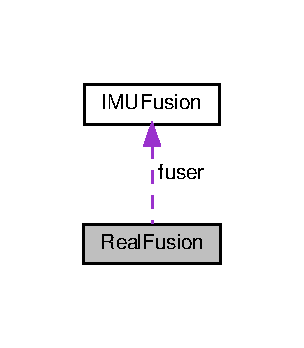
\includegraphics[width=146pt]{classRealFusion__coll__graph}
\end{center}
\end{figure}
\subsection*{Public Member Functions}
\begin{DoxyCompactItemize}
\item 
\hyperlink{classRealFusion_a9632f71572a51d7db415793e1976a958}{Real\+Fusion} ()  throw (\+Exception)
\begin{DoxyCompactList}\small\item\em Default Constructor. \end{DoxyCompactList}\item 
bool \hyperlink{classRealFusion_a77329f8bfa4390754ddb1c72b58281ff}{check\+I\+MU} ()
\begin{DoxyCompactList}\small\item\em Checks availability of I\+MU. \end{DoxyCompactList}\item 
void \hyperlink{classRealFusion_a0fa5b36d1b32622ec65c41e2c3852c2f}{tick} ()
\begin{DoxyCompactList}\small\item\em Performs the fusion. \end{DoxyCompactList}\end{DoxyCompactItemize}
\subsection*{Public Attributes}
\begin{DoxyCompactItemize}
\item 
\mbox{\Hypertarget{classRealFusion_ab67b42c3cc2f4dffefa894d96b82751b}\label{classRealFusion_ab67b42c3cc2f4dffefa894d96b82751b}} 
Fusion\+Euler\+Angles {\bfseries angles}
\end{DoxyCompactItemize}
\subsection*{Protected Attributes}
\begin{DoxyCompactItemize}
\item 
\mbox{\Hypertarget{classRealFusion_aa8e9a57cb02c2151f3783e88f8e0b662}\label{classRealFusion_aa8e9a57cb02c2151f3783e88f8e0b662}} 
rs2\+::pipeline {\bfseries pl}
\item 
\mbox{\Hypertarget{classRealFusion_a041aa40f221d98af87b4ebfc0138b83a}\label{classRealFusion_a041aa40f221d98af87b4ebfc0138b83a}} 
\hyperlink{classIMUFusion}{I\+M\+U\+Fusion} {\bfseries fuser}
\end{DoxyCompactItemize}


\subsection{Detailed Description}
A class to encapsulate librealsense2 and Fusion access. 



\subsection{Constructor \& Destructor Documentation}
\mbox{\Hypertarget{classRealFusion_a9632f71572a51d7db415793e1976a958}\label{classRealFusion_a9632f71572a51d7db415793e1976a958}} 
\index{Real\+Fusion@{Real\+Fusion}!Real\+Fusion@{Real\+Fusion}}
\index{Real\+Fusion@{Real\+Fusion}!Real\+Fusion@{Real\+Fusion}}
\subsubsection{\texorpdfstring{Real\+Fusion()}{RealFusion()}}
{\footnotesize\ttfamily Real\+Fusion\+::\+Real\+Fusion (\begin{DoxyParamCaption}{ }\end{DoxyParamCaption}) throw  \hyperlink{classException}{Exception}) }



Default Constructor. 

Checks I\+MU available, initializes librealsense. 

\subsection{Member Function Documentation}
\mbox{\Hypertarget{classRealFusion_a77329f8bfa4390754ddb1c72b58281ff}\label{classRealFusion_a77329f8bfa4390754ddb1c72b58281ff}} 
\index{Real\+Fusion@{Real\+Fusion}!check\+I\+MU@{check\+I\+MU}}
\index{check\+I\+MU@{check\+I\+MU}!Real\+Fusion@{Real\+Fusion}}
\subsubsection{\texorpdfstring{check\+I\+M\+U()}{checkIMU()}}
{\footnotesize\ttfamily bool Real\+Fusion\+::check\+I\+MU (\begin{DoxyParamCaption}{ }\end{DoxyParamCaption})}



Checks availability of I\+MU. 

\begin{DoxyReturn}{Returns}
true if I\+MU exists, false if not 
\end{DoxyReturn}
\mbox{\Hypertarget{classRealFusion_a0fa5b36d1b32622ec65c41e2c3852c2f}\label{classRealFusion_a0fa5b36d1b32622ec65c41e2c3852c2f}} 
\index{Real\+Fusion@{Real\+Fusion}!tick@{tick}}
\index{tick@{tick}!Real\+Fusion@{Real\+Fusion}}
\subsubsection{\texorpdfstring{tick()}{tick()}}
{\footnotesize\ttfamily void Real\+Fusion\+::tick (\begin{DoxyParamCaption}{ }\end{DoxyParamCaption})}



Performs the fusion. 

Retrieves frames from librealsense2, extracts I\+MU data, and calls Fusion to perform Madgwick fusion to obtain Euler orientation which it caches in the angles public member. \begin{DoxyReturn}{Returns}
void 
\end{DoxyReturn}


The documentation for this class was generated from the following files\+:\begin{DoxyCompactItemize}
\item 
\hyperlink{RealFusion_8hpp}{Real\+Fusion.\+hpp}\item 
\hyperlink{RealFusion_8cpp}{Real\+Fusion.\+cpp}\end{DoxyCompactItemize}

\chapter{File Documentation}
\hypertarget{IMUFusion_8cpp}{}\section{I\+M\+U\+Fusion.\+cpp File Reference}
\label{IMUFusion_8cpp}\index{I\+M\+U\+Fusion.\+cpp@{I\+M\+U\+Fusion.\+cpp}}


Fuse\+To\+Euler shows how to incorporate Sebastian Madgwick\textquotesingle{}s sensor fusion library to fuse raw I\+MU gyroscope and accelerometer telemetry from Real\+Sense cameras.  


{\ttfamily \#include \char`\"{}I\+M\+U\+Fusion.\+hpp\char`\"{}}\newline
Include dependency graph for I\+M\+U\+Fusion.\+cpp\+:\nopagebreak
\begin{figure}[H]
\begin{center}
\leavevmode
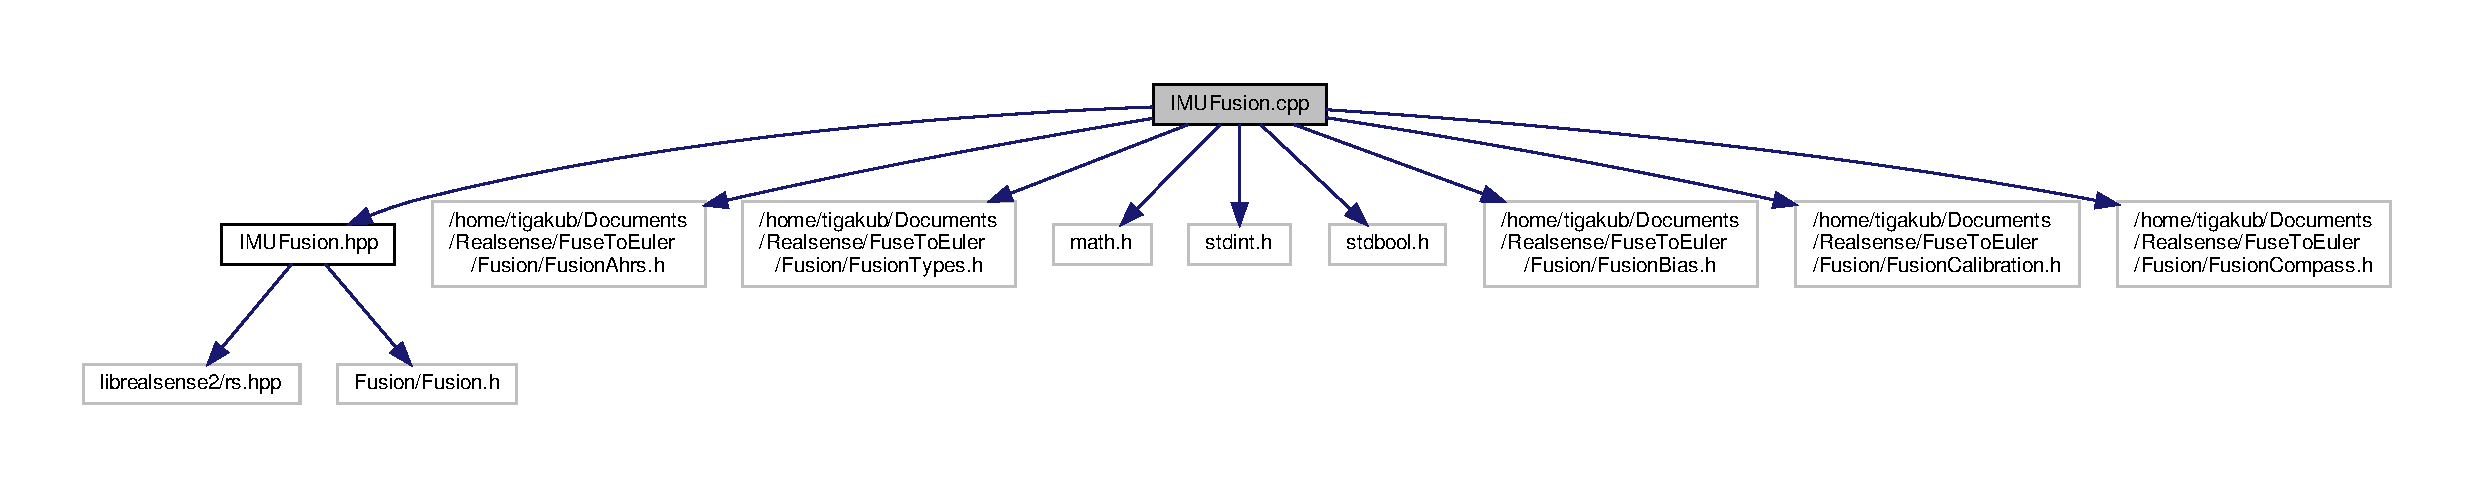
\includegraphics[width=350pt]{IMUFusion_8cpp__incl}
\end{center}
\end{figure}


\subsection{Detailed Description}
Fuse\+To\+Euler shows how to incorporate Sebastian Madgwick\textquotesingle{}s sensor fusion library to fuse raw I\+MU gyroscope and accelerometer telemetry from Real\+Sense cameras. 

\begin{DoxyCopyright}{Copyright}
Copyright (C) 2021 Edward Janne -\/ All Rights Reserved
\end{DoxyCopyright}
\hypertarget{RealFusion_8hpp_LICENSE}{}\subsection{L\+I\+C\+E\+N\+SE}\label{RealFusion_8hpp_LICENSE}
This file is part of Fuse\+To\+Euler.

Fuse\+To\+Euler is free software\+: you can redistribute it and/or modify it under the terms of the G\+NU General Public License as published by the Free Software Foundation, either version 3 of the License, or (at your option) any later version.

Fuse\+To\+Euler is distributed in the hope that it will be useful, but W\+I\+T\+H\+O\+UT A\+NY W\+A\+R\+R\+A\+N\+TY; without even the implied warranty of M\+E\+R\+C\+H\+A\+N\+T\+A\+B\+I\+L\+I\+TY or F\+I\+T\+N\+E\+SS F\+OR A P\+A\+R\+T\+I\+C\+U\+L\+AR P\+U\+R\+P\+O\+SE. See the G\+NU General Public License for more details.

You should have received a copy of the G\+NU General Public License along with Fuse\+To\+Euler. If not, see \href{https://www.gnu.org/licenses/}{\tt https\+://www.\+gnu.\+org/licenses/}.

\begin{DoxyAuthor}{Author}
Edward Janne 
\end{DoxyAuthor}

\hypertarget{IMUFusion_8hpp}{}\section{I\+M\+U\+Fusion.\+hpp File Reference}
\label{IMUFusion_8hpp}\index{I\+M\+U\+Fusion.\+hpp@{I\+M\+U\+Fusion.\+hpp}}


Fuse\+To\+Euler shows how to incorporate Sebastian Madgwick\textquotesingle{}s sensor fusion library to fuse raw I\+MU gyroscope and accelerometer telemetry from Real\+Sense cameras.  


{\ttfamily \#include $<$librealsense2/rs.\+hpp$>$}\newline
{\ttfamily \#include \char`\"{}Fusion/\+Fusion.\+h\char`\"{}}\newline
Include dependency graph for I\+M\+U\+Fusion.\+hpp\+:\nopagebreak
\begin{figure}[H]
\begin{center}
\leavevmode
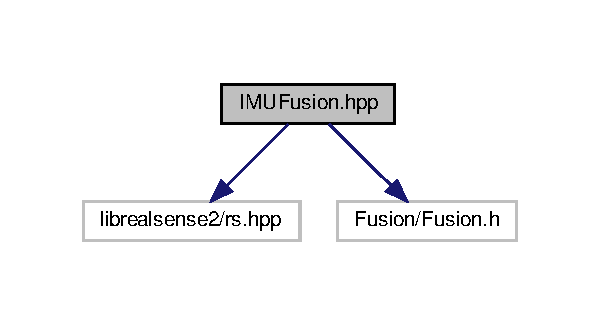
\includegraphics[width=288pt]{IMUFusion_8hpp__incl}
\end{center}
\end{figure}
This graph shows which files directly or indirectly include this file\+:\nopagebreak
\begin{figure}[H]
\begin{center}
\leavevmode
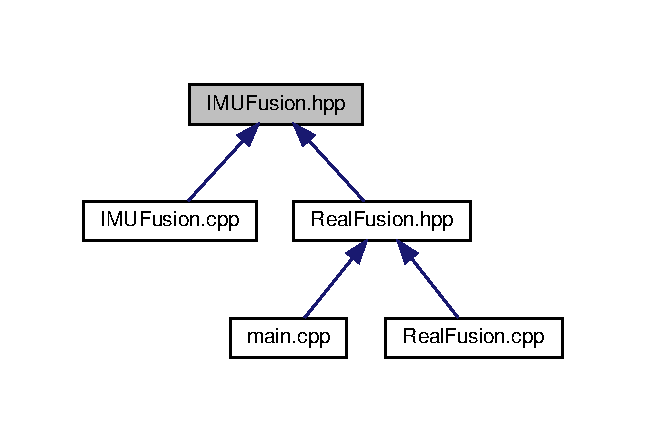
\includegraphics[width=310pt]{IMUFusion_8hpp__dep__incl}
\end{center}
\end{figure}
\subsection*{Classes}
\begin{DoxyCompactItemize}
\item 
class \hyperlink{classIMUFusion}{I\+M\+U\+Fusion}
\begin{DoxyCompactList}\small\item\em A class to encapsulate Madgwick Fusion access. \end{DoxyCompactList}\end{DoxyCompactItemize}
\subsection*{Macros}
\begin{DoxyCompactItemize}
\item 
\mbox{\Hypertarget{IMUFusion_8hpp_a6e58fcea626847c9734cdc19eb93a6c5}\label{IMUFusion_8hpp_a6e58fcea626847c9734cdc19eb93a6c5}} 
\#define {\bfseries G\+Y\+R\+O\+\_\+\+S\+E\+N\+S\+I\+T\+I\+V\+I\+TY}~262.\+144f
\item 
\mbox{\Hypertarget{IMUFusion_8hpp_a09ecf77e46d9d12697d484dcb1a54842}\label{IMUFusion_8hpp_a09ecf77e46d9d12697d484dcb1a54842}} 
\#define {\bfseries A\+C\+C\+E\+L\+\_\+\+S\+E\+N\+S\+I\+T\+I\+V\+I\+TY}~16384.\+0f
\end{DoxyCompactItemize}


\subsection{Detailed Description}
Fuse\+To\+Euler shows how to incorporate Sebastian Madgwick\textquotesingle{}s sensor fusion library to fuse raw I\+MU gyroscope and accelerometer telemetry from Real\+Sense cameras. 

\begin{DoxyCopyright}{Copyright}
Copyright (C) 2021 Edward Janne -\/ All Rights Reserved
\end{DoxyCopyright}
\hypertarget{RealFusion_8hpp_LICENSE}{}\subsection{L\+I\+C\+E\+N\+SE}\label{RealFusion_8hpp_LICENSE}
This file is part of Fuse\+To\+Euler.

Fuse\+To\+Euler is free software\+: you can redistribute it and/or modify it under the terms of the G\+NU General Public License as published by the Free Software Foundation, either version 3 of the License, or (at your option) any later version.

Fuse\+To\+Euler is distributed in the hope that it will be useful, but W\+I\+T\+H\+O\+UT A\+NY W\+A\+R\+R\+A\+N\+TY; without even the implied warranty of M\+E\+R\+C\+H\+A\+N\+T\+A\+B\+I\+L\+I\+TY or F\+I\+T\+N\+E\+SS F\+OR A P\+A\+R\+T\+I\+C\+U\+L\+AR P\+U\+R\+P\+O\+SE. See the G\+NU General Public License for more details.

You should have received a copy of the G\+NU General Public License along with Fuse\+To\+Euler. If not, see \href{https://www.gnu.org/licenses/}{\tt https\+://www.\+gnu.\+org/licenses/}.

\begin{DoxyAuthor}{Author}
Edward Janne 
\end{DoxyAuthor}

\hypertarget{main_8cpp}{}\section{main.\+cpp File Reference}
\label{main_8cpp}\index{main.\+cpp@{main.\+cpp}}


Fuse\+To\+Euler shows how to incorporate Sebastian Madgwick\textquotesingle{}s sensor fusion library to fuse raw I\+MU gyroscope and accelerometer telemetry from Real\+Sense cameras.  


{\ttfamily \#include $<$iostream$>$}\newline
{\ttfamily \#include $<$csignal$>$}\newline
{\ttfamily \#include $<$chrono$>$}\newline
{\ttfamily \#include $<$atomic$>$}\newline
{\ttfamily \#include \char`\"{}Real\+Fusion.\+hpp\char`\"{}}\newline
Include dependency graph for main.\+cpp\+:\nopagebreak
\begin{figure}[H]
\begin{center}
\leavevmode
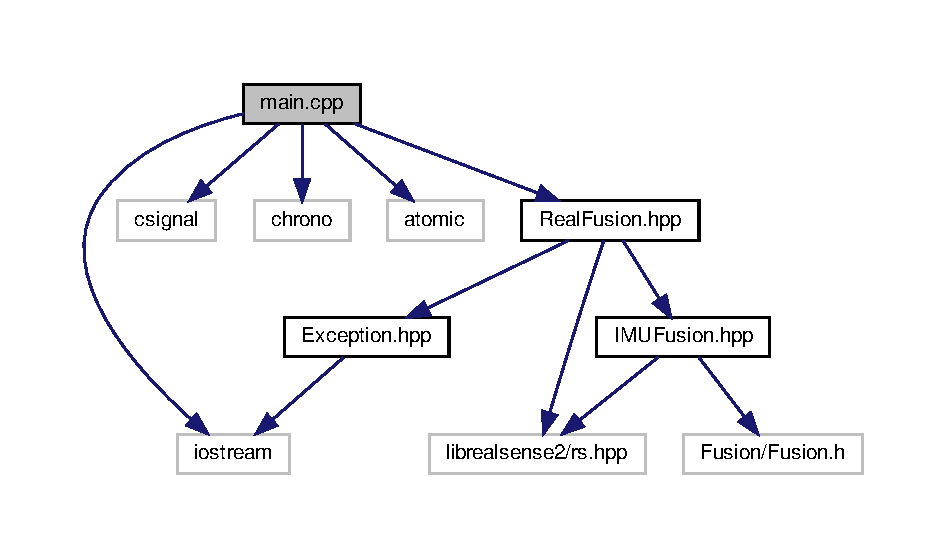
\includegraphics[width=350pt]{main_8cpp__incl}
\end{center}
\end{figure}
\subsection*{Functions}
\begin{DoxyCompactItemize}
\item 
\mbox{\Hypertarget{main_8cpp_a9b99e599116053d9c4debd54231d2868}\label{main_8cpp_a9b99e599116053d9c4debd54231d2868}} 
void {\bfseries sigint\+Handler} (int i\+Sig\+Num)
\item 
\mbox{\Hypertarget{main_8cpp_a3c04138a5bfe5d72780bb7e82a18e627}\label{main_8cpp_a3c04138a5bfe5d72780bb7e82a18e627}} 
int {\bfseries main} (int argc, char $\ast$$\ast$argv)
\end{DoxyCompactItemize}
\subsection*{Variables}
\begin{DoxyCompactItemize}
\item 
\mbox{\Hypertarget{main_8cpp_ad87b684fbf7e057a5c08e1b0016dfe79}\label{main_8cpp_ad87b684fbf7e057a5c08e1b0016dfe79}} 
atomic$<$ bool $>$ {\bfseries alive} \{true\}
\end{DoxyCompactItemize}


\subsection{Detailed Description}
Fuse\+To\+Euler shows how to incorporate Sebastian Madgwick\textquotesingle{}s sensor fusion library to fuse raw I\+MU gyroscope and accelerometer telemetry from Real\+Sense cameras. 

\begin{DoxyCopyright}{Copyright}
Copyright (C) 2021 Edward Janne -\/ All Rights Reserved
\end{DoxyCopyright}
\hypertarget{RealFusion_8hpp_LICENSE}{}\subsection{L\+I\+C\+E\+N\+SE}\label{RealFusion_8hpp_LICENSE}
This file is part of Fuse\+To\+Euler.

Fuse\+To\+Euler is free software\+: you can redistribute it and/or modify it under the terms of the G\+NU General Public License as published by the Free Software Foundation, either version 3 of the License, or (at your option) any later version.

Fuse\+To\+Euler is distributed in the hope that it will be useful, but W\+I\+T\+H\+O\+UT A\+NY W\+A\+R\+R\+A\+N\+TY; without even the implied warranty of M\+E\+R\+C\+H\+A\+N\+T\+A\+B\+I\+L\+I\+TY or F\+I\+T\+N\+E\+SS F\+OR A P\+A\+R\+T\+I\+C\+U\+L\+AR P\+U\+R\+P\+O\+SE. See the G\+NU General Public License for more details.

You should have received a copy of the G\+NU General Public License along with Fuse\+To\+Euler. If not, see \href{https://www.gnu.org/licenses/}{\tt https\+://www.\+gnu.\+org/licenses/}.

\begin{DoxyAuthor}{Author}
Edward Janne 
\end{DoxyAuthor}

\hypertarget{RealFusion_8cpp}{}\section{Real\+Fusion.\+cpp File Reference}
\label{RealFusion_8cpp}\index{Real\+Fusion.\+cpp@{Real\+Fusion.\+cpp}}


Fuse\+To\+Euler shows how to incorporate Sebastian Madgwick\textquotesingle{}s sensor fusion library to fuse raw I\+MU gyroscope and accelerometer telemetry from Real\+Sense cameras.  


{\ttfamily \#include \char`\"{}Real\+Fusion.\+hpp\char`\"{}}\newline
Include dependency graph for Real\+Fusion.\+cpp\+:\nopagebreak
\begin{figure}[H]
\begin{center}
\leavevmode
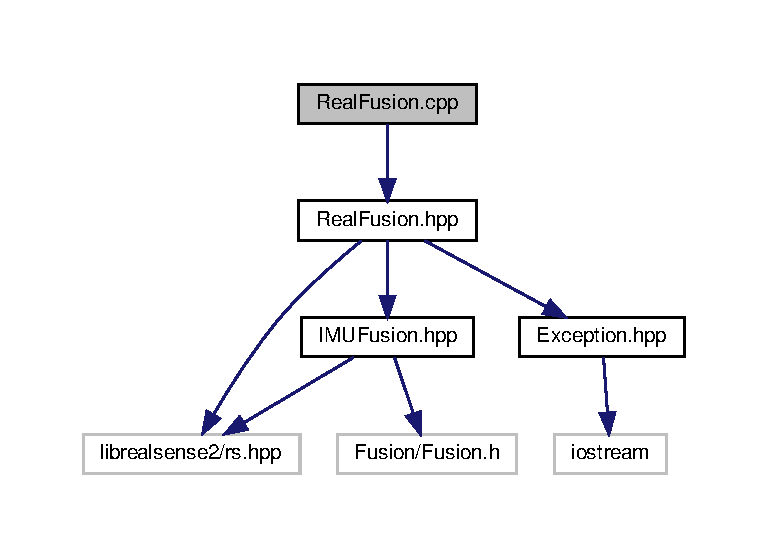
\includegraphics[width=350pt]{RealFusion_8cpp__incl}
\end{center}
\end{figure}


\subsection{Detailed Description}
Fuse\+To\+Euler shows how to incorporate Sebastian Madgwick\textquotesingle{}s sensor fusion library to fuse raw I\+MU gyroscope and accelerometer telemetry from Real\+Sense cameras. 

\begin{DoxyCopyright}{Copyright}
Copyright (C) 2021 Edward Janne -\/ All Rights Reserved
\end{DoxyCopyright}
\hypertarget{RealFusion_8hpp_LICENSE}{}\subsection{L\+I\+C\+E\+N\+SE}\label{RealFusion_8hpp_LICENSE}
This file is part of Fuse\+To\+Euler.

Fuse\+To\+Euler is free software\+: you can redistribute it and/or modify it under the terms of the G\+NU General Public License as published by the Free Software Foundation, either version 3 of the License, or (at your option) any later version.

Fuse\+To\+Euler is distributed in the hope that it will be useful, but W\+I\+T\+H\+O\+UT A\+NY W\+A\+R\+R\+A\+N\+TY; without even the implied warranty of M\+E\+R\+C\+H\+A\+N\+T\+A\+B\+I\+L\+I\+TY or F\+I\+T\+N\+E\+SS F\+OR A P\+A\+R\+T\+I\+C\+U\+L\+AR P\+U\+R\+P\+O\+SE. See the G\+NU General Public License for more details.

You should have received a copy of the G\+NU General Public License along with Fuse\+To\+Euler. If not, see \href{https://www.gnu.org/licenses/}{\tt https\+://www.\+gnu.\+org/licenses/}.

\begin{DoxyAuthor}{Author}
Edward Janne 
\end{DoxyAuthor}

\hypertarget{RealFusion_8hpp}{}\section{Real\+Fusion.\+hpp File Reference}
\label{RealFusion_8hpp}\index{Real\+Fusion.\+hpp@{Real\+Fusion.\+hpp}}


Fuse\+To\+Euler shows how to incorporate Sebastian Madgwick\textquotesingle{}s sensor fusion library to fuse raw I\+MU gyroscope and accelerometer telemetry from Real\+Sense cameras.  


{\ttfamily \#include $<$librealsense2/rs.\+hpp$>$}\newline
{\ttfamily \#include \char`\"{}I\+M\+U\+Fusion.\+hpp\char`\"{}}\newline
{\ttfamily \#include \char`\"{}Exception.\+hpp\char`\"{}}\newline
Include dependency graph for Real\+Fusion.\+hpp\+:\nopagebreak
\begin{figure}[H]
\begin{center}
\leavevmode
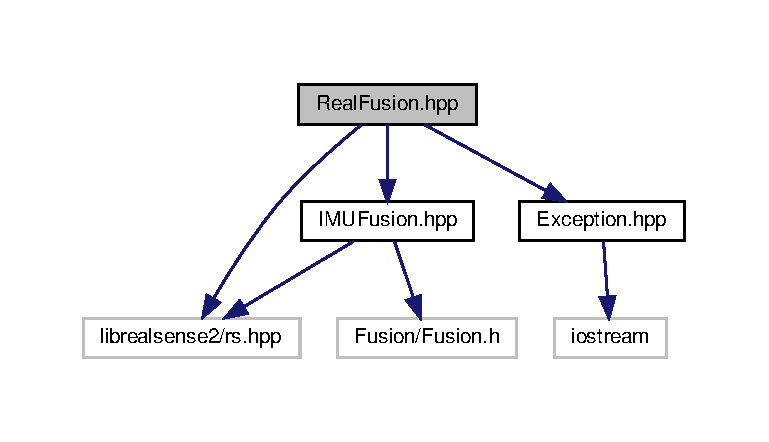
\includegraphics[width=350pt]{RealFusion_8hpp__incl}
\end{center}
\end{figure}
This graph shows which files directly or indirectly include this file\+:\nopagebreak
\begin{figure}[H]
\begin{center}
\leavevmode
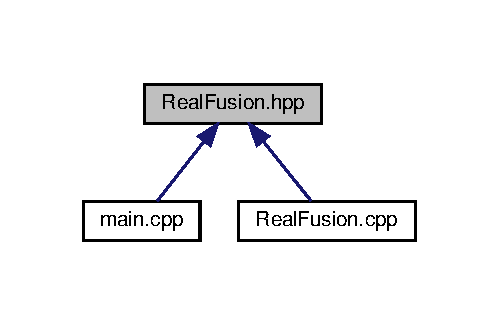
\includegraphics[width=240pt]{RealFusion_8hpp__dep__incl}
\end{center}
\end{figure}
\subsection*{Classes}
\begin{DoxyCompactItemize}
\item 
class \hyperlink{classRealFusion}{Real\+Fusion}
\begin{DoxyCompactList}\small\item\em A class to encapsulate librealsense2 and Fusion access. \end{DoxyCompactList}\end{DoxyCompactItemize}


\subsection{Detailed Description}
Fuse\+To\+Euler shows how to incorporate Sebastian Madgwick\textquotesingle{}s sensor fusion library to fuse raw I\+MU gyroscope and accelerometer telemetry from Real\+Sense cameras. 

\begin{DoxyCopyright}{Copyright}
Copyright (C) 2021 Edward Janne -\/ All Rights Reserved
\end{DoxyCopyright}
\hypertarget{RealFusion_8hpp_LICENSE}{}\subsection{L\+I\+C\+E\+N\+SE}\label{RealFusion_8hpp_LICENSE}
This file is part of Fuse\+To\+Euler.

Fuse\+To\+Euler is free software\+: you can redistribute it and/or modify it under the terms of the G\+NU General Public License as published by the Free Software Foundation, either version 3 of the License, or (at your option) any later version.

Fuse\+To\+Euler is distributed in the hope that it will be useful, but W\+I\+T\+H\+O\+UT A\+NY W\+A\+R\+R\+A\+N\+TY; without even the implied warranty of M\+E\+R\+C\+H\+A\+N\+T\+A\+B\+I\+L\+I\+TY or F\+I\+T\+N\+E\+SS F\+OR A P\+A\+R\+T\+I\+C\+U\+L\+AR P\+U\+R\+P\+O\+SE. See the G\+NU General Public License for more details.

You should have received a copy of the G\+NU General Public License along with Fuse\+To\+Euler. If not, see \href{https://www.gnu.org/licenses/}{\tt https\+://www.\+gnu.\+org/licenses/}.

\begin{DoxyAuthor}{Author}
Edward Janne 
\end{DoxyAuthor}

%--- End generated contents ---

% Index
\backmatter
\newpage
\phantomsection
\clearemptydoublepage
\addcontentsline{toc}{chapter}{Index}
\printindex

\end{document}
